\section{Process' Perspective}
\label{sec:processPerspective}

\subsection{Overview}
\label{subsec:overview}
The main focus of the \hyperref[sec:processPerspective]{Process' Perspective section} will be how code and artifacts go from idea to production and which tools and processes are involved?\\
\hyperref[subsec:TeamInteraction]{2.2 Team Interaction and Organization} will discuss communication within the team. \hyperref[subsec:cicd]{2.3 CI/CD chains} will reason for the choice of CI/CD platform and take a deeper look and both CI and CD chains.
\hyperref[subsec:vs]{2.4 Version Control} discusses strategies related to the way version control is used and managed. These include repository setup and branching strategy. In 
\hyperref[subsec:process&tools]{2.5 Development process and tools} we discuss how issues and projects were used to track, label, and assign tasks within the team.
\hyperref[subsec:monitoring]{2.6 Monitoring And Logs} will introduce the Prometheus Grafana stack and the elk stack and what value these have brought to service.
\hyperref[subsec:security]{2.7 Security} will be a brief rundown of results from the security analysis and pentest, and an introduction to the techniques used for secret handling.
The final section \hyperref[subsec:scaling]{2.8 Scaling And Load balancing} will focus on the migration from single server architecture to a Kubernetes cluster and provide a discussion on some of the pros and cons of using Kubernetes for scaling and load balancing.

\subsection{Team Interaction and Organization}
\label{subsec:TeamInteraction}
Most internal planning and communication have gone through \href{https://discord.com/}{Discord}. The team has a server with text channels for planning, resources etc. Work has been split between remote using discord voice channels and physical at and in continuation of the allotted exercise time on Tuesdays.
\subsection{CI/CD chains}
\label{subsec:cicd}
% github workflows
% - A complete description of stages and tools included in the CI/CD chains.
% That is, including deployment and release of your systems.

Utilizing a CI/CD pipeline allows us to test, build, and deploy the MiniTwit service incrementally with minimal manual interference. Thus, saving us a significant amount of time setting up environments, allowing us to deploy fast and often while still being able to revert to an earlier version quickly.
It provides us with ways of measuring and improving the quality of all code coming from local development to version control and eventually reaching production, and by that reduces human error.\footnote{Continuous delivery: Huge benefits, but challenges too\cite{Chen2015}}
In essence, an automated CI/CD pipeline puts multiple DevOps ideas into practice: 
\begin{itemize}
    \item Flow (Keeping batch sizes small)\footnote{\label{handbook}The DevOps handbook\cite{Kim2016}} 
    \item Feedback (Instant, rapid and continuous feedback on code entering pipeline)\footnote{The DevOps handbook\cite{Kim2016}}
\end{itemize}


\subsubsection{CI/CD Platform}
\label{subsubsec:cicdPlatform}
An abundance of CI/CD platforms are available to developers. Our CI/CD chains are set up using GitHub Actions. GitHub Actions integrates seamlessly with our GitHub repositories and allows us to trigger workflows every time an event occurs in a repository\footnote{Understanding GitHub Actions\cite{githubActions}}. Many other providers such as Travis CI\href{https://travis-ci.org/}{travisCI} or TeamCity\href{https://www.jetbrains.com/teamcity/}{TeamCity} offer these same features and some even more, but not for free and not with little to no initial configuration. However, we are not blind to concerns with using the same provider for most tools. The most notable of these would be more considerable consequences when GitHub inevitably goes offline or experiences problems. We accept these concerns as we prefer the ease of use and price tag over distributing our tools and having a smaller chance of being impaired due to provider outages.

\subsubsection{CI - Continuous Integration}
\label{subsubsec:ci}
As illustrated in \hyperref[fig:CIStateMachine]{Figure 1}, the entry point for the CI pipeline is creating a pull request to the main branch, which will trigger several GitHub Actions workflows.
\begin{enumerate}
    \item \textbf{.Net Build and test} - The backbone of the CI pipeline, which compiles, builds, and tests the backend. It provides us immediate feedback on whether the changes run and passes the test suite. When implementing the backend, we spent a significant amount of time and effort setting up a test suite comprised of unit tests and integration tests, which allows us to trust that this workflow will catch breaking change coming into the codebase.
    \item \textbf{Quality analysis tools} - These tools all provide feedback on the quality of the pushed code per their definition of code quality. These include .Net analyzers, Sonarcloud, Better Code Hub, and DeepScan.
    \item \textbf{Dependency scanning tools} - Scans dependencies and codebase for security hazards and fails if the security gate specified to "Critical" severity is met. These include snyk and CodeQL.
\end{enumerate}


\begin {figure}[H]
    \centering
    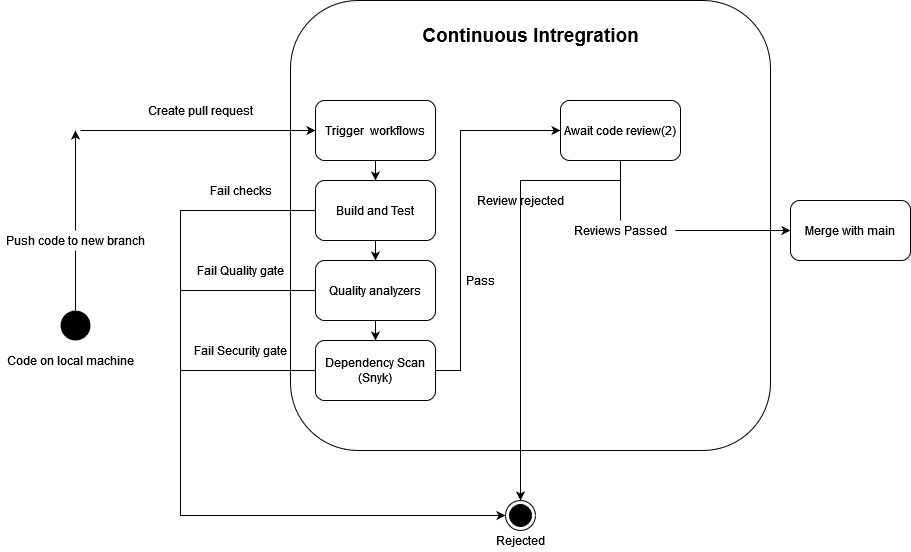
\includegraphics[scale=0.50]{images/DevopsDiagrams-StateMachine CI.drawio(4).png}
    \caption{CI Pipeline State Machine Diagram}
    \label{fig:CIStateMachine}
\end{figure}
As suggested by \hyperref[fig:CIStateMachine]{figure 1}, if any of these fail, the CI pipeline will direct to a rejected state, from where a developer can fix problems, push to the rejected branch, and the workflows will rerun. Once all workflows are passed, the pull request awaits review until at least two team members have approved it. From here, changes can be merged into the main branch.

\subsubsection{CD - Continuous Delivery/Deployment}
\label{subsubsec:cd}

Our pipeline introduces a mix of Continuous Delivery and Continuous Deployment(Illustrated in \hyperref[fig:CDStateMachine]{Figure 2}). Deployment is done entirely by the deployment workflow(cluster-deploy.yml).
The workflow is triggered every time a release is created. It also supports manual dispatch for hot fixing errors, and the weekly release workflow runs every Sunday evening, triggering the deployment pipeline. The deployment workflow is comprised of 4 jobs.
\begin{enumerate}
    \item \textbf{.Net Build and Test} - This job is described in \hyperref[subsubsec:ci]{CI - Continuous Integration}.
    \item \textbf{Build and Push containers} - Builds docker containers for the frontend and backend, tags them with proper versions, then pushes them to docker hub. This allows us to keep our Operations repository lean as we can then pull all necessary containers from docker hub.
    \item \textbf{Snyk Dependency scan} - Our security gate. If a risk exceeding the gate is found, the deployment will stop immediately and move to the canceled state. See \hyperref[fig:CDStateMachine]{Figure 2}
    \item \textbf{Dispatch} - Dispatches the apply workflow in the Operations repository.
\end{enumerate}

\begin {figure}[H]
    \centering
    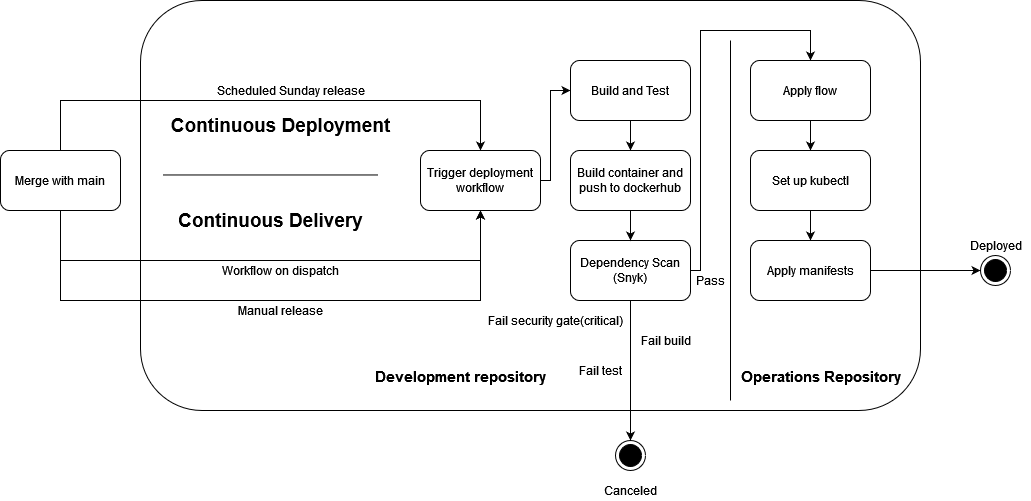
\includegraphics[scale=0.50]{images/DevopsDiagrams-StateMachineCd.drawio.png}
    \caption{CD Pipeline State Machine Diagram}
    \label{fig:CDStateMachine}
\end{figure}

When checks have passed and the apply workflow has been dispatched, the runner will set up kubectl using a Digital ocean token, with the cluster name saved as secrets in the repository. With access to kubectl, the runner now has access to the Kubernetes cluster. The apply shell script is executed, which "applies" all the configuration manifests, thus deploying the changes.


\subsection{Version Control}
\label{subsec:vs}
% Organization of your repositor(ies).
% That is, either the structure of of mono-repository or organization of artifacts across repositories.
% In essence, it has to be be clear what is stored where and why
\subsubsection{Organization of Repositories}
%Do we use a single or multi repo setup. --> we Use submodules and automatic steps for updating them
% Draft: feel free to edit/ delete
\subsubsection{Branching Strategy}
%branching STRATEGY:
%Can't push to main, need two reviewers on a pull request
%Need one review on pull requests to production
% Trunk based - stuff on main are in a working state

% - Applied branching strategy.
% For example, how did you use issues, Kanban boards, etc. to organize open tasks

Our organization uses a Trunk Based Development branching model. We have two centralized branches, which were continuously debugged, tested, and in a working state. Features, patches, and bug fixes are always developed on dedicated temporary branches, which are deleted after being merged into their relative centralized branch. \\

\textbf{\hyperref[app:devRepo]{Dev Repository} @ main} \\\\
The \textbf{main} branch lives on GitHub and is the alpha of our centralized workflow. While we develop features and patches on temporary branches, everything worthwhile is eventually merged into main. \\

Primary applications of the main branch are:
\begin{enumerate}
    \item Store our working source code
    \item Make releases
    \item Run workflows
    \item Build and push docker images\\
\end{enumerate}

\textbf{\hyperref[app:opsRepo]{Ops Repository} @ master}\\\\
The master branch of the Ops repository contains infrastructure as code for creating and configuring a Kubernetes cluster with \href{https://www.digitalocean.com/}{DigitalOcean} as provider, manifest files used to deploy our service to the cluster, and shell scripts for automating these steps. It is developed in a manner such that our multi-container application can be rebuilt and updated to include updated Docker images and changes in configuration files requiring minimal effort.

\subsection{Development process and tools}
\label{subsec:process&tools}
% - Applied development process and tools supporting it
GitHub issues track what needs to be done and how far a task is from completion. Upon creation, issues are tagged and organized into GitHub Projects. By using a combination of issues, projects, and enforcement of code reviews, we promote transparency between developers, thus making sure to spread progress and knowledge of the codebase between multiple developers.

\subsection{Monitoring And Logs}
\label{subsec:monitoring}
%kibana and grafana
%metrics
% How do you monitor your systems and what precisely do you monitor?
% What do you log in your systems and how do you aggregate logs?

\subsection{Security}
\label{subsec:security}
To discover, define, and asses vulnerabilities of our system, we have conducted a security assessment and a pen-test. This section will include only select results. The rest is available in \hyperref[app:secAss]{Secuirity Assesment section of the Appendix}.

Using the \href{https://owasp.org/Top10/}{OWASP Top 10} we identified possible insecurities in our system. We constructed risk scenarios and analyzed their likelihood and impact. 
The analysis yielded "Outdated Components" as a top concern. As security breaches on are discovered half a year later on average, the way to combat security threats is proactivity\footnote{Security lecture. Add citation}. To decrease chance of having outdated components in production, we added dependabot to our GitHub repository and snyk to our CI chain. Dependabot creates pull requests automatically suggesting updates to outdated components. Snyk scans the repository for dependencies with vulnerabilities. It also scans for sensitive data leaks. Handling of secrets to prevent such leaks will be described in the \hyperref[subsubsec:secrets]{Secret Handling} section.
We also conducted an automated penetration test to:
\begin{enumerate}
    \item Detect vulnerabilities
    \item Test the system under stress.
\end{enumerate}
Using the logging system, we noticed that the server received requests from all around the world, e.g. Nevada. In conclusion, except for acting as a DOS attack on our own system, eventually crashing the ELK stack. The pen test did not yield any system vulnerabilities.

\subsubsection{Secret Handling}
\label{subsubsec:secrets}
Securing sensitive data while allowing access to multiple parties is a challenging ordeal.

\subsection{Scaling And Load balancing}
\label{subsec:scaling}
% Applied strategy for scaling and load balancing.
%Include reflection over why scaling and load balancing benefit us, why kubernetes might have been overkill for the project, but which pros and cons we considered when deciding.

\subsubsection{Single server setup}
\label{subsubsec:scalingProd}
The original single server setup that was deployed on a digital ocean droplet using docker-compose is located on \textbf{\hyperref[app:devRepo]{Dev Repository} @ production}
Although now deprecated, the production branch had our production server and was our main branch's lean and automated counterpart. It was developed in a manner such that our multi-container application could be rebuilt and updated on the production server to include updated Docker images and changes in configuration files with a single command, minimizing downtime without using load-balancers.\\
Although cheap and easy to set up. The original single-server architecture had several shortcomings if we were to handle additional traffic while minimizing downtime.
Only vertical scaling using the digital ocean API was possible. This approach has multiple downsides. It will become exceedingly more expensive as more virtual CPU cores, RAM, and disk space is added, eventually reaching an upper limit. The single monolithic VM will forever be a single point of failure, and upgrading the VM will require the server to shut down.
(MAYBE INCLUDE COMPONENT DIAGRAM)

\subsubsection{Scaling the application}
\label{subsubsec:scalingApp}
In order to scale for handling additional traffic while minimizing downtime, the team had a couple of options. Eliminating the server as a single point of failure while allowing for rolling updates out without shutting down the application could be accomplished by introducing a setup with a primary server and backup server while swapping around IPs, but that would not allow for horizontal scaling.\\
Options that, out of the box, come with horizontal scaling, load balancing, and rolling updates while eliminating the single point of failure could be container orchestration tools like Docker Swarm and Kubernetes.\\ 
We have chosen to migrate our application to a Kubernetes cluster. There is an argument that the additional complexity and setup required for deploying a Kubernetes cluster is unnecessary since Docker Swarm fulfills our requirements, thus conflicting with the simplicity principle. After all according to the agile manifesto, "Simplicity--the art of maximizing the amount
of work not done--is essential"\footnote{(Beck, et al., 2001)\cite{beck2001agile}}. The first reason for the choice is that documentation on the setup and management of a Kubernetes cluster was a lot more extensive, although the increased complexity might cause that. Secondly, the team wished to gain experience using Kubernetes for container orchestration. That said, automated scaling\footnote{https://kubernetes.io/} does save time for developers, even if monitoring service load and manually scaling a swarm when required is a possible solution. In conclusion, by migrating to a Kubernetes cluster, we support horizontal scaling, load balancing, and rolling updates. However, we must admit that even though the database was flushed and deployed to the cluster, we do not have a replicated database because of consistency concerns and can therefore not claim to have eliminated all single points of failure.
